
\section{SDL2 Game Structure}
\label{sec:SDL2-Game-Structure-section}

% Give me the basic structure of the game using SDL2
In this section, we will explore the fundamental structure of our SDL2-based poker game. The game follows a standard SDL2 application architecture with the following key components:

\begin{itemize}
    \item \textbf{Initialization}: Setting up SDL2, creating windows and renderers
    \item \textbf{Game Loop}: The main loop that handles:
        \begin{itemize}
            \item Event handling (user input)
            \item Game state updates
            \item Rendering
        \end{itemize}
    \item \textbf{Resource Management}: Loading and managing textures, fonts, and sounds
    \item \textbf{Cleanup}: Proper deallocation of resources
\end{itemize}

\subsection{Core Components}
The game is structured around several core classes:

\begin{itemize}
    \item \texttt{Game}: Main class managing the game state and loop
    \item \texttt{TextureManager}: Handles loading and rendering of images
    \item \texttt{InputHandler}: Processes user input
    \item \texttt{Player}: Manages player data and actions
    \item \texttt{Card}: Represents individual playing cards
    \item \texttt{Deck}: Handles the deck of cards and dealing
\end{itemize}

Figure \ref{fig:game-structure} illustrates the relationship between these components.

\begin{figure}[h]
    \centering
    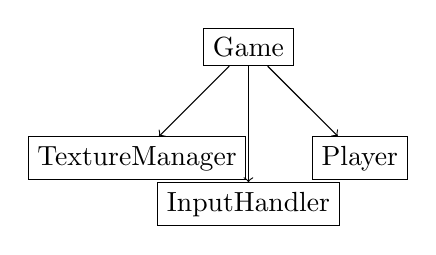
\begin{tikzpicture}[node distance=2cm]
        \node[rectangle,draw] (game) {Game};
        \node[rectangle,draw] (texture) [below left of=game] {TextureManager};
        \node[rectangle,draw] (input) [below of=game] {InputHandler};
        \node[rectangle,draw] (player) [below right of=game] {Player};
        
        \draw[->] (game) -- (texture);
        \draw[->] (game) -- (input);
        \draw[->] (game) -- (player);
    \end{tikzpicture}
    \caption{Basic game structure diagram}
    \label{fig:game-structure}
\end{figure}

